\section*{Analysis}
\label{analysis}

It is possible to look at a spider plot in order to get a sense of how the speakers were rated overall. For example the BeoLab 5 overall scores the highest in the attributes: \textit{Flashy}, \textit{Decorated}, \textit{Wide}, \textit{Untypical}. This seems reasonable when presented with the speakers next to each other in \autoref{fig:speakers}. 
\begin{figure}
\centering
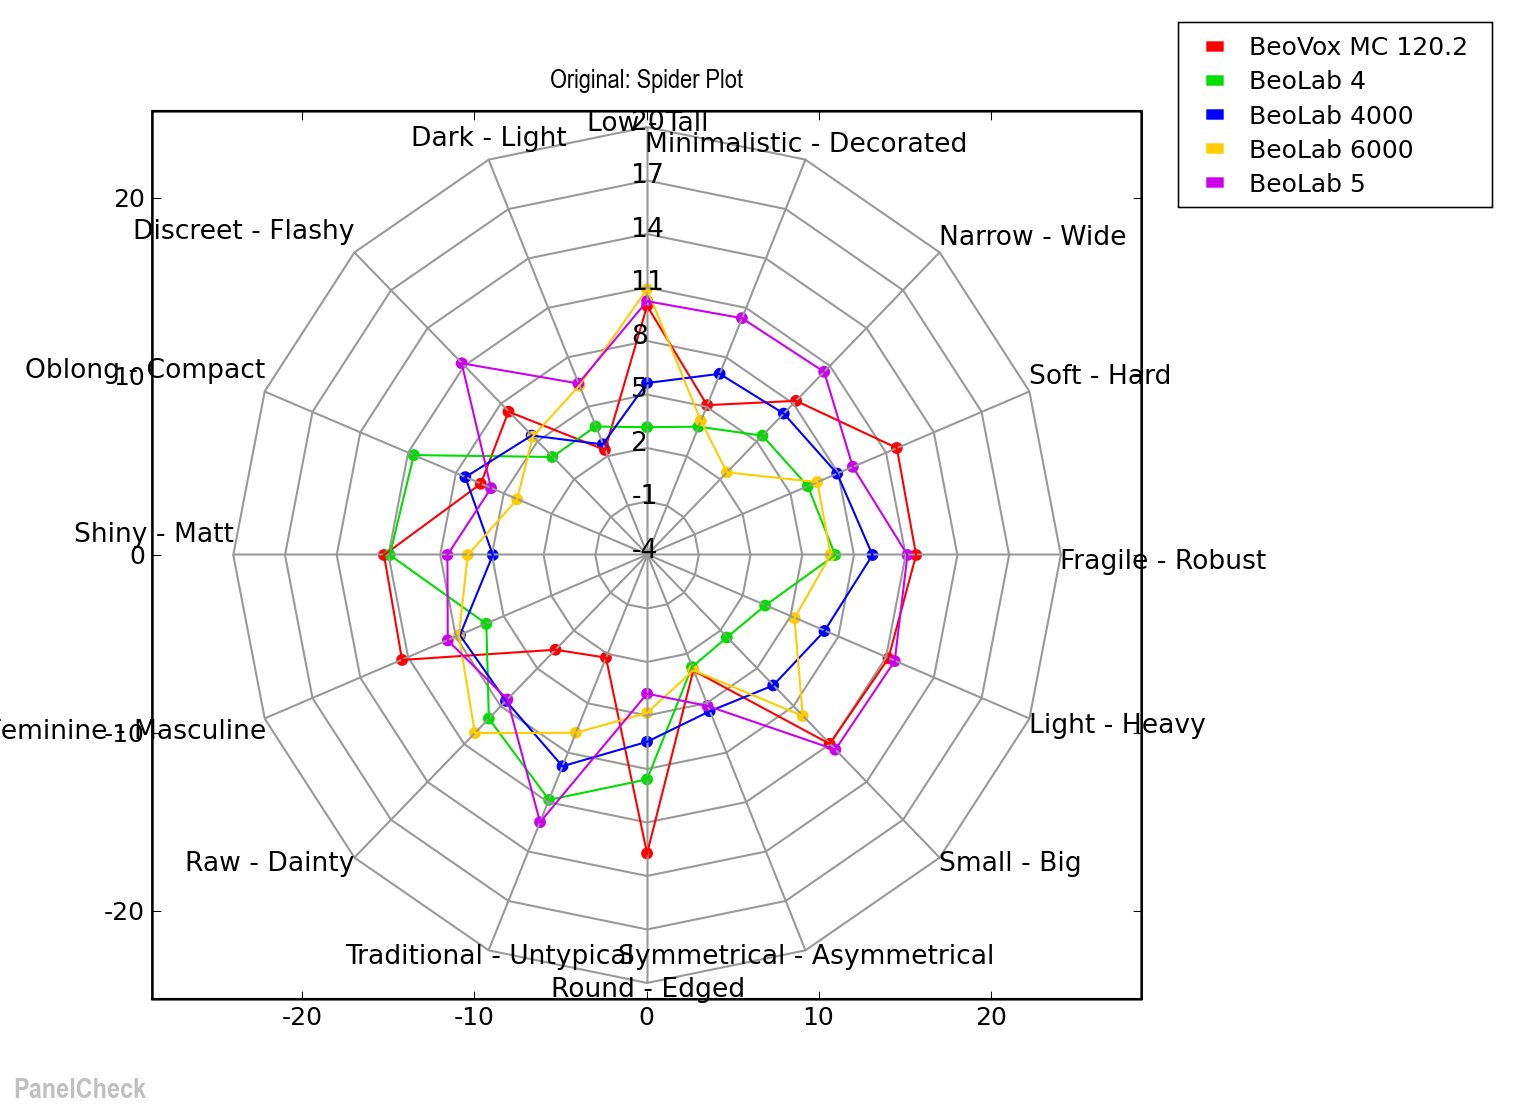
\includegraphics[width = \textwidth]{Figure/spider_plot.png}
\caption{A spider plot of the subjects' preference of the five different speakers}
\label{fig:spider_plot}
\end{figure}